\section{Continuous phase transitions}

In order to address the behavior of a system during a continuous phase transition we can imagine to work in a situation like the one of an unstable binary material. In that case we have that the system wants to generate areas in two different phases and since it's unstable as it is the process that will go through in forming them is a continuous transformation that naturally generates gradients of concentration inside the material. On a more general level we can say that the concentration is the order parameter $\xi$ inside the material and the transformation is naturally generating a gradient $\grad \xi$ inside the system that we want to study. 
\begin{figure}[b]
    \centering
    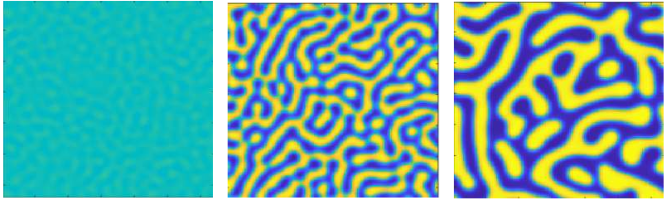
\includegraphics[width=0.8\textwidth]{Immagini/ContPhaseTrans.png}
    \caption{
        Result of a simulation to represent a phase transition in a binary alloy showing in different colors different densities that can be interpreted as the order parameter of the system.
    }
    \label{fig:ContPhaseTrans}
\end{figure}
A great example of this is shown in \figref{fig:ContPhaseTrans}, where the material starts from an ordered situation with uniform density to then naturally create domains generating disorder.

To study such a phenomenon we should not focus our attention only on the domain that are forming inside the material, but an important contribution to the free energy is given by the interfacial regions. The latter are the region of space where the system goes from one domain to another, so the position where $\grad \xi$ is effectively large and non-zero. In fact, such interfaces have a large role in the creation of the new phases since their number is really large in the first part of the transformation driving it at its core. Still, the presence of a gradient needs to generate an increase of $G(\xi)$ due to the fact that the minima of the free energy are represented by the order parameter in the domain, $\xi_\alpha$ and $\xi_\beta$. This means that, for $\xi$ in between those two, present in the wall domain composing the interfaces, necessarily has higher free energy overall increasing it. Therefore, one may ask why they exist and are not reduced to the minimum, and the reason for it can be understood by making the example of magnetic domain in a ferromagnetic material. We know how the gain in energy inside a magnetic domain is due to \textbf{exchange interaction} between spins that prefers to have aligned spin minimizing the energy and increase it otherwise. In this situation having two domains with opposite spins one next to the other highly increase the energy, so that the presence of a gradient that smooth out the interaction is favorable. The question then becomes, how large should such interface be in order for it be effectively be energetically favorable giving rise to the generation of the domains, and how do they evolve? That's the question we are going to answer right now.

\subsection{Cahn-Hilliard equation}

To start modelling the evolution of the system during a phase transition we need to write down a form for the free energy focussing on the local free energy, that we will call $f^{hom}$. We will assume that such a function will depend on the order parameter and it's gradient, allowing us to write down a Taylor expansion of it near the value of $\grad \xi = 0$
\begin{equation}
    f(\xi, \grad\xi) = f^{hom}(\xi) + \pdv{f^{hom}}{\grad \xi}\vdot \grad\xi + \pdv[2] {f^{hom}}{\grad \xi} \grad\xi \vdot \grad \xi.
\end{equation}
We can simplify such a form by noticing that if we change variable $\xi \to -\xi$ also the gradient change sign having that the first order term will modify the energy of the system. That is an absurd since a simple change of variable can't change the physics of the system having that the first derivative respect to the gradient needs to be zero. We can then define $K$ as the second derivative term to end up with the following form
\begin{equation}
    \label{eq:LocalFreeEnerg}
    f(\xi, \grad\xi) = f^{hom}(\xi) + K\grad \xi^2.
\end{equation}
The two terms present behaves so that the first wants to eliminate interfaces since works simply as the local free energy, meaning that has minima for the values of $\xi$ corresponding to the domains and increase as the order changes. Instead, the second term goes against that pushing for the creation of larger interfaces so that $\grad\xi$ is more extended but lower in absolute value along the material. In fact, if no interface would be present the gradient between two domains would have $\abs{\grad\xi} \to \infty$ rising a lot the value of the second term.

Therefore, the \eqref{eq:LocalFreeEnerg} will allow us to model the behavior of the system in general giving us insights on the form of the interfaces. As a matter of facts, it's possible to use such a form to arrive at the following simple result.
\thm{Interface properties}
{
    Inside a continuous phase transformation where the local free energy can be written as in \eqref{eq:LocalFreeEnerg} the width of the domain interfaces and the surface free energy are given by
    \begin{align}
        &\delta = \sqrt{\frac{K}{\mean{f^{hom}}}}, &\gamma = 2\sqrt{K\mean{f^{hom}}}.
    \end{align}
}
\pf{Proof}
{
    We can write down the total energy in the proximity of an interface by integrating the local free energy so that
    \begin{equation}
        F = \int_V \left[ f^{hom}(\xi) + K\left( \dv{\xi}{x} \right)^2 \right]\dd V,
    \end{equation}
    where we assumed that the interface is only in direction $x$ so that the gradient is present only in that component. We can then average the quantity over the volume of the interface by multipling and dividing for $A\delta$, where $A$ is the area of the interface and $\delta$ the width
    \begin{equation}
        F = A\delta\left[ \mean{f^{hom}} + K \mean{\left( \dv{\xi}{x} \right)^2} \right].
    \end{equation}
    The width of the interface can then be set to $\delta \approx \dd x/\dd\xi$ having that the final form of the energy is
    \begin{equation}
        F \approx A\left[ \mean{f^{hom}}\delta + \frac{K}{\delta} \right].
    \end{equation}
    By minimizing this value one can find the wanted value of the width that minimize the free energy and then by substitute it inside $F$ and dividing it by $A$ also $\gamma$ can be computed.
}
\noindent
This is the result we expected after the previous description of the energy. In fact, we can see that as the parameter $K$, related to the gradient term, increase the width of the interfaces inside the material, while the average value of $f^{hom}$ decrease them, exactly as we said before.

% TODO: Vai direttamente con l'equazione di Cahn-Hiliard, non perdere tempo.